\section{Experiments}
\label{sec:campaign}

We executed \NCampaignPairs{} (defense, attack) pairs across \NCampaignImpl{}
defense implementations and \NCampaignEpisodes{} scored episodes. Every
method ran from its authors' released code and weights.
Figure~\ref{fig:transfer} sets the campaign beside the published literature.

\begin{figure}[t]
\centering
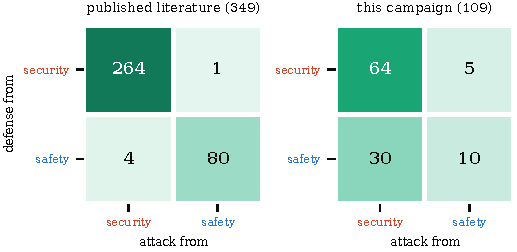
\includegraphics[width=\columnwidth]{figures/fig6_transfer}
\caption{Who built the defense (rows) against whose problem it was run
(columns). Left, every confirmed pair in the literature; right, every pair
in this campaign. Shade is each cell's share of its own panel, so the two
panels are not on one colour scale and the printed count is the value. The
literature crosses between the communities in \NCrossCommunityPairs{} pairs
of \NPureRegimePairs{} (\PctCrossCommunity{}\%); one of its two
off-diagonal boxes holds a single pair. All four boxes are occupied on the
right.}
\label{fig:transfer}
\end{figure}

The main experiment puts a defense from one literature in front of an attack
from the other. We ran \NCampCrossPairs{} such pairs, all on retrieval
question answering over Natural Questions.
\NCampSafDefSecMech{} of them take a knowledge-conflict method, built for a
document that is merely out of date, and attack it with corpus poisoning,
PoisonedRAG or BadRAG. The remaining \NCampSecDefSafetyMech{} run the other
way: a defense built against an attacker meets a failure nobody wrote, such
as a passage retrieved for the wrong question or a real passage whose answer
has since changed.

A second experiment pairs each method with the kind of attack its own authors
used. These \NCampSecDefSecMech{} security pairs and
\NCampSafDefSafetyMech{} safety pairs tell us nothing about whether a method
carries across, and we ran them so that a failure in the paragraph above
cannot be blamed on our harness. Most of them are the agent experiment:
\NAgentPairs{} pairs in which eight prompt-injection defenses meet seven
injected-instruction attacks inside the AgentDojo banking
suite~\cite{debenedetti-2024-agentdojo}.

A third experiment holds the defense and the dose fixed and changes only the
shape of the planted passage. The five shapes are a token sequence optimized
to be retrieved, a fluent sentence asserting the answer the model would have
given from memory, the same sentence asserting a third answer instead, a real
passage retrieved for another question, and a real passage with its answer
swapped. A defense that behaves differently across them is keying on the
shape of the text rather than on the attack it was named for.

A fourth set of runs supplies the measurements published evaluations leave
out. Every run above carries three arms on the same items: a clean arm with
nothing planted, an undefended arm, and an arm that sees no document at all.
We also re-ran the retrieval experiment on a second base model, and we ran
both released implementations of the one defense design that held, which
share a principle and no code downstream of it.

The last two experiments test the explanation rather than the methods. We
built two attacks against the single defense that resisted, one searching
over surface forms and one optimizing a suffix with gradients, both targeting
the quantity that defense's own rule measures. And we stacked two defenses
that act at different stages of the same pipeline, to test the design rule
the observations below arrive at.
